% Example LaTeX document for GP111 - note % sign indicates a comment
\documentclass[12pt]{article}
% Default margins are too wide all the way around. I reset them here
\usepackage{amsmath}
%\usepackage{mathtools}
\usepackage{graphicx}
\usepackage[danish]{babel}
\usepackage{listings}
\usepackage{color}
\usepackage[utf8]{inputenc}
\usepackage{hyperref}
\usepackage{float}

\definecolor{lightgray}{rgb}{.9,.9,.9}
\definecolor{darkgray}{rgb}{.4,.4,.4}
\definecolor{purple}{rgb}{0.65, 0.12, 0.82}

\lstdefinelanguage{JavaScript}{
	keywords={typeof, new, true, false, catch, function, return, null, catch, switch, var, if, in, while, do, else, case, break, eval, getElementById},
	keywordstyle=\color{blue}\bfseries,
	ndkeywords={class, export, boolean, throw, implements, import, this, document},
	ndkeywordstyle=\color{darkgray}\bfseries,
	identifierstyle=\color{black},
	sensitive=false,
	comment=[l]{//},
	morecomment=[s]{/*}{*/},
	commentstyle=\color{purple}\ttfamily,
	stringstyle=\color{red}\ttfamily,
	morestring=[b]',
	morestring=[b]"
}

\lstset{
	language=JavaScript,
	backgroundcolor=\color{lightgray},
	extendedchars=true,
	basicstyle=\footnotesize\ttfamily,
	showstringspaces=false,
	showspaces=false,
	numbers=left,
	numberstyle=\footnotesize,
	numbersep=9pt,
	tabsize=2,
	breaklines=true,
	showtabs=false,
	captionpos=t
}

\renewcommand\lstlistingname{Funktion}
\addto{\captionsdanish}{\renewcommand{\abstractname}{Abstract}}
\numberwithin{equation}{section}

\pagestyle{headings}

\begin{document}
\title{Numerisk Integration}
\author{Søren Fritzbøger 3F\\
HTX Hillerød - Erhversskolen Nordsjælland\\
Vejleder: Stig og CHR}
\renewcommand{\today}{2. Februar 2015}
\maketitle

\begin{abstract}
This article demonstrates a basic set of LaTeX formatting commands.
Compare the typeset output side-by-side with the input document.smøøre
\end{abstract}
\newpage
\tableofcontents
\newpage
\section{Indledning}

\section{Forklaring af numerisk integration}



\section{Trapezmetoden}
\label{sec:trapezmetoden}
Trapezmetoden er en af flere metoder til at finde areal under en funktion. Det er en af de mere præcise metoder, da den, i modsætning til højre-, venstre- og middelsum, laver en trapez og ikke en firkant.
\subsection{Bevis for trapezmetoden}
Ved at bruge trapezmetoden kan vi tilnærmelsesvist finde det bestemte integral, selv for funktioner, hvor man ikke direkte kan bestemme det bestemte integral. Et eksempel på dette er funktionen $f(x)=e^{-x^{2}}$.
For at bestemme arealet under en funktion vil vi gerne nærme os det bestemte integral.
\begin{equation}
\int_{a}^{b}f(x)dx \nonumber
\end{equation}
Når $a<b$ og $f$ er kontinuerlig og differentiabel i intervallet $[a;b]$, kan vi bruge trapezmetoden til at udregne det tilnærmelsesvist bestemte integral, som er arealet under funktionen.\\
Som navnet trapezmetoden så fint hentyder til, opdeler vi vores funktion i en trapez, som vi udregner arealet af. Dette er illustreret på figur \ref{fig:trapezmetoden}
\begin{figure}[H]
\centering
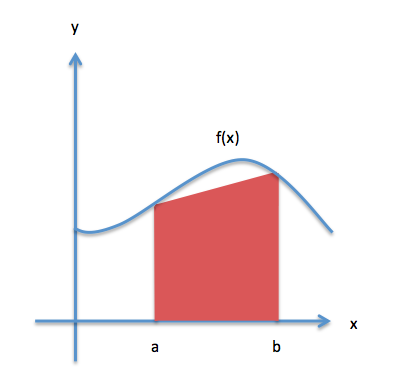
\includegraphics[scale=0.5]{Billeder/trapezmetoden.png}
\caption{Trapezmetoden}
\label{fig:trapezmetoden}
\end{figure}


På figur \ref{fig:trapezmetoden} kan man se, hvordan trapezmetoden opdeler en parabel i en trapez. Denne trapez har intervallet $[a;b]$. Længden $a=f(a)$ og længden $b=f(b)$. Formlen for arealet af en trapez ses i formel \eqref{eq:trapezareal}
\begin{equation}
\label{eq:trapezareal}
A=\frac{1}{2}h\cdot(a+b)
\end{equation}
\begin{figure}[H]
	\centering
	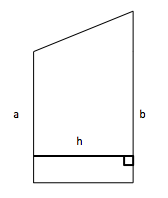
\includegraphics[scale=0.6]{Billeder/Trapez}
	\caption{Trapez}
	\label{fig:trapez}
\end{figure}

Som man kan se på figur \ref{fig:trapez}, er $a$ og $b$ er sidelænger og $h$ er højden. I et trapez er højden defineret som afstanden mellem de to parallelle linjestykker, i dette tilfælde $a$ og $b$, som man kan se illustreret på figur \ref{fig:trapez}
\\\\
Som man kan se på figur \ref{fig:trapez} svarer højden $h$ til afstanden mellem $a$ og $b$, som svarer til $h=b-a$. Når man indsætter henholdsvis $a$ og $b$ værdien ind i vores $f(x)$ funktion, får vi vores $y$ værdi, som svarer til længden af henholdsvis $a$ og $b$.
Hvis vi indsætter dette i arealet for en trapez, får vi derfor:
\begin{align}
A &= \frac{1}{2}h\cdot(a+b) &\Rightarrow \nonumber
\\ &= \frac{1}{2}(b-a) \cdot (a+b) &\Rightarrow \nonumber
\\ &= \frac{b-a}{2} (a+b) &\Rightarrow \nonumber
\intertext{i stedet for $a$ og $b$ indsættes højderne på trapezens sider, $f(a)$ og $f(b)$} \nonumber
\\ &= \frac{b-a}{2} (f(a)+f(b))
\\ \intertext{Arealet af denne trapez svarer tilnærmelsesvist til arealet under funktionen. Så derfor kan vi sige at arealet af trapezen tilnærmelsesvist svarer til værdien af det bestemte integral:} \nonumber
\\ \int_{a}^{b}f(x) &\approx \frac{b-a}{2} (f(a)+f(b))
\end{align}

\subsubsection{Opdeling i flere delintervaller}
\label{sec:opdelingtrapezmetoden}
Som man kan se på figur \ref{fig:trapezmetoden} er trapezmetoden meget upræcis i forhold til det bestemte integral. Dette kan man forbedre ved at dele intervallet $[a;b]$ op i flere delintervaller, $n$. Dvs. at vi deler vores funktion op i mindre intervaller, som vi så finder arealet af med trapezmetoden. Disse delintervaller kalder vi for $x_0, x_1, \cdots x_n$. Vi skal bruge højden på trapezen, som er længden af delintervallet $x_0 - x_1$. I dette tilfælde svarer det til:
\begin{align}
h = x_1-x_0 = x_2-x_1 = \cdots = x_n - x_{n-1}
\end{align}
Ud fra dette kan vi bestemme at højden, $h$, må svare til intervallet $[a;b]$ opdelt i $n$ intervaller:
\begin{align}
h=\frac{b-a}{n}
\end{align}
Det samlede areal under funktionen kan betegnes som summen af alle delintervallerne:
\begin{align}
A &= \lim\limits_{n \rightarrow \infty} \sum_{i=1}^{n} \frac{h}{2}(f(x_{i}) + f(x_{i+1}))
\approx \int_{a}^{b}f(x) &\text{hvor }h=\frac{b-a}{n}
\end{align}
Når n går mod uendelig bliver vores delinterval infinitesimalt lille, hvilket vil sige at summen af alle trapezarealerne nærmer sig det bestemte integral. Det bestemte integral svarer faktisk til at vi deler arealet op i uendelige små og uendelig mange led.
\\\\
For at udlede dette til formlen for trapezmetoden bliver vi nødt til at opskrive dette på en lidt anden måde.
\begin{align}
A &= \frac{h}{2}(f(x_0)+ f(x_1)) + \frac{h}{2}(f(x_1)+ f(x_2)) + \cdots + \frac{h}{2}(f(x_{n-1})+ f(x_n)) \nonumber
\\ &= h(\frac{1}{2}f(x_0) + \frac{1}{2}f(x_1)) + h(\frac{1}{2}f(x_1) + \frac{1}{2}f(x_2)) + \cdots + h(\frac{1}{2}f(x_{n-1}) + \frac{1}{2}f(x_n)) \nonumber
\\ &= h \cdot \frac{1}{2}f(x_0) + h \cdot \frac{1}{2}f(x_1) + h \cdot \frac{1}{2}f(x_1) + h \cdot \frac{1}{2}f(x_2) + \cdots + h \cdot \frac{1}{2}f(x_{n-1}) + h \cdot \frac{1}{2}f(x_n) \nonumber
\end{align}
Dette bliver reduceret til formlen for trapezmetoden \eqref{eq:trapezmetoden}
\begin{align}
\label{eq:trapezmetoden}
\boxed{\int_{a}^{b}f(x) \approx \frac{h}{2}(f(x_0) + 2f(x_1) + \cdots + 2f(x_{n-1}) + f(x_n))} \\ \text{Hvor } h=\frac{b-a}{n} \nonumber
\end{align}

\section{Simpsons metode}
\label{sec:simpsonsmetode}
En anden metode til tilnærmelsesvist at udregne arealet under en funktion er simpsons-metoden, som virker ved at dele funktionen op i mindre parabler, man så finder arealet under. Denne metode er mere præcis end trapezmetoden\footnote{\cite[side 15]{2012matA}}, og giver derfor et resultat som oftest har en meget lille afvigelse fra det korrekte resultat, det bestemte integral.
\subsection{Bevis for Simpsons metode}
Simpsons metode er som nævnt, en anden metode til tilnærmelsesvist at finde det bestemte integral, selv for funktioner, hvor man ikke direkte kan bestemme det bestemte integral. Med trapezmetoden, se afsnit \ref{sec:trapezmetoden}, brugte man en ret linje fra $f(a)$ til $f(b)$ i intervallet $[a;b]$, hvilket selvfølgelig ikke er helt præcis, da en funktion ikke nødvendigvis er ret. Med Simpsons metode opdeler man intervallet $[a;b]$ i en parabel ud fra 3 punkter, $a,b,c$. Disse tre punkter kan bruges til at opstille en simplere parabel, som vi så kan regne arealet under. Parablens ligning ser således ud: $y=ax^2+bx+c$
\begin{figure}[H]
\centering
\includegraphics[width=0.6\linewidth]{Billeder/Simpsonsmetode}
\caption{Simpsons metode}
\label{fig:simpsonsmetode}
\end{figure}

Figur \ref{fig:simpsonsmetode} viser hvilke punkter vores parabel går gennem når vi har intervallet $[a;b]$. Ligesom med trapezmetoden kan man opdele funktionen i $n$ antal dele. Til at starte med går vi ud fra at $n=2$, for at gøre det nemt.\emph{I afsnit \ref{sec:simpsonopdeling} bliver der viderebygget på Simpsons metode med flere intervaller.}
Som man også kan se på figuren bliver $[a;b]$ delt op i to, hvor $\triangle x=h$. Dette viser sig også i punkterne som henholdsvis er $(-h,y_0)$, $(0,y_1)$ og $(h,y_2)$. Intervallet $[a;b]$ opdeles i $n$ antal delintervaller, som for dette tilfælde er 2, hvilket giver afstanden h mellem vores punkter.
\begin{align}
h &= \frac{b-a}{n} \nonumber
\\&= \frac{b-a}{2} &\text{Når } n=2
\end{align}
Vi ved at vores parabel går fra $-h$ til $h$ og at den har forskriften $y=ax^2+bx+c$. Dette simple udtryk for vores parabel kan vi bestemme det bestemte integral af, da vi ved at $f(x)=y$. Vi finder dermed det bestemte areal under en parabel med forskriften $y=ax^2+bx+c$ fra $-h$ til $h$
\begin{align}
\label{eq:integral-hh}
A &=\int_{-h}^{h}f(x)dx \nonumber
\\ &=\left[ \frac{ax^3}{3} + \frac{bx^2}{2} + cx \right]_{-h}^{h} \nonumber
\\ &= \left( \frac{ah^3}{3} + \frac{bh^2}{2} + ch \right) - \left( -\frac{ah^3}{3} + \frac{bh^2}{2} - ch \right) \nonumber
\\ &= \frac{ah^3}{3} + \frac{ah^3}{3} + \frac{bh^2}{2} - \frac{bh^2}{2} + ch + ch \nonumber
\\ &= \frac{2ah^3}{3} + 2ch \nonumber
\\ &= \frac{h}{3}(2ah^2+6c)
\end{align}

Nu skal vi finde vores 2 ubekendte, som er $2ah^2$ og $c$. Dette kan vi gøre ved at opstille tre ligninger for parablen, $y=ax^2+bx+c$, med vores tre punkter $(-h,y_0)$, $(0,y_1)$, $(h,y_2)$ fra figur \ref{fig:simpsonsmetode}, hvor vi så har 3 ubekendte. Vi går ud fra at $y$ svarer til punkternes y-koordinat og $x$ til vores x-koordinat.

\begin{align}
\label{eq:ubekendte}
y_0 &= ah^2-bh+c & \text{Hvor } (x,y) &=(-h,y_0)
\\ y_1 &= a \cdot 0^2+b \cdot 0 +c \Rightarrow \nonumber
\\ y_1 &= c & \text{Hvor } (x,y) &=(0,y_1)
\\ y_2 &= ah^2+bh+c & \text{ } (x,y) &=(h,y_2)
\end{align}
Som man kan se på ligningen for $y_1$ \eqref{eq:ubekendte} har vi allerede fået isoleret vores $c$ værdi, som svarer til $c=y_1$
Vi vil gerne have isoleret $2ah^2$, og dette kan vi gøre ved at substituere $c$ ind i de to ligninger for $y_0$ og $y_2$ og derefter ligge dem sammen.
\\\\
Det gør vi således:
\begin{align}
y_0 &= ah^2 - bh + c &\Rightarrow &&\text{Hvor } c=y_1 \nonumber
\\ y_0 &= ah^2 -bh + y_1 & \Rightarrow \nonumber
\\ y_0-y_1 &= ah^2-bh
\label{eq:ah2-bh}
\\ \nonumber
\\y_2 &= ah^2 + bh + c &\Rightarrow &&\text{Hvor } c=y_1 \nonumber
\\y_2 &= ah^2 + bh + y_1 & \Rightarrow \nonumber
\\y_2 - y_1 &= ah^2 +bh
\label{eq:ah2+bh}
\end{align}
Ligning \eqref{eq:ah2-bh} og \eqref{eq:ah2+bh} ligges nu sammen, så vi kan isolere den sidste og manglende ubekendte, $2ah^2$.

\begin{align}
	y_2 - y_1 &= ah^2 - bh &+ \nonumber
\\	y_0 - y_1 &= ah^2 + bh \nonumber
\\ &&= \nonumber
\\ ah^2 -bh + bh &= y_2 + y_0 - y_1 - y_1 \Rightarrow \nonumber
\\ ah^2 &= y_2 + y_0 - 2y_1
\end{align}
$ah^2$ og $c$ substitueres nu ind i formel \eqref{eq:integral-hh} som ser således ud: $A = \frac{h}{3}(2ah^2+6c).$

\begin{align}
\label{eq:ensimpson}
A &= \frac{h}{3}(2ah^2+6c) \nonumber
\\&= \frac{h}{3}\left( \left( y_2+y_0-2y_1 \right) + 6 \cdot y_1 \right) \nonumber
\\&= \frac{h}{3}(y_0+4y_1+y_2)
\end{align}


%Ud fra ligning \eqref{integral-hh} kan vi lave vores parabel ved at opstille tre ligninger med 3 ubekendte, vha. vores 3 punkter: $(-h,y_0)$, $(0,y_1)$, $(h,y_2)$.
%De tre ligninger ser således ud:

\subsubsection{Opdeling i flere delintervaller}
Når vi deler vores interval op i flere delintervaller, dvs. at $n$ bliver større, kan vi finde summen af $n$ antal delintervaller mellem $[a;b]$. På figur \ref{fig:simpsonOpdeling} kan man se et eksempel på en opdeling med $n=2$, hvor vi faktisk har 2 parabler. En fra $y_0$ til $y_2$ gennem $y_1$ og en fra $y_2$ til $y_4$ gennem $y_3$.
\label{sec:simpsonopdeling}
\begin{figure}[H]
\centering
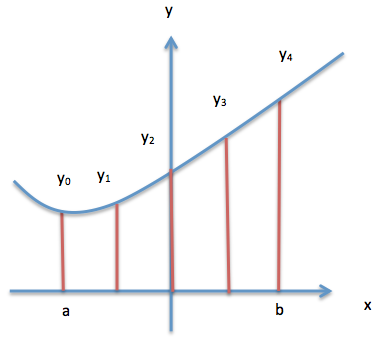
\includegraphics[width=0.6\linewidth]{Billeder/simpsonOpdeling}
\caption{Opdeling i flere delintervaller}
\label{fig:simpsonOpdeling}
\end{figure}

Ved hjælp af formel \eqref{eq:ensimpson} kan vi udregne arealet af en parabel fra $y_0$ til $y_2$. Men hvis vi udvider denne som man kan se på figur \ref{fig:simpsonOpdeling}, kan vi fortsætte simpsonsreglen fra $y_2$ til $y_4$, og dermed få det samlede areal for $[a;b]$ som går fra $y_0$ til $y_4$, som man kan se på figur \ref{fig:simpsonOpdeling}.
Summen af arealet fra $[a;b]$ når opdelingen $n=4$
\begin{align}
\label{eq:simpsonOpdeling}
A_{[a;b]} 	&= \frac{h}{3}(y_0 + 4y_1 + y_2) + \frac{h}{3}(y_2 + 4y_3 + y_4) \nonumber
\\ 			&= \frac{h}{3}(y_0 + 4y_1 + y_2 + y_2 +4y_3 +y_4) \nonumber
\\			&= \frac{h}{3}(y_0 + 4y_1 + 2y_2 + 4y_3 + y_4) & \text{Hvor } y=f(x)
\intertext{Det samme sker hvis vi har en opdeling på $n=6$}
A_{[a;b]}	&= \frac{h}{3}(y_0 + 4y_1 + 2y_2 + 4y_3 + 2y_4 + 4y_5 + y_6) & \text{Når } n=6
\label{eq:simpsonOpdeling6}
\end{align}
Ud fra dette kan vi opstille en ligning der siger at summen af alle delarealerne i intervallet $[a;b]$ opdelt i $n$ delintervaller tilnærmelsesvist må svare til det bestemte integral.
\begin{align}
A &= \lim\limits_{n \rightarrow \infty} \sum_{i=1}^{n/2} \frac{h}{3}(y_{i-2} + 4y_{i-1} + y_{i}) \approx \int_{a}^{b}f(x) &\text{hvor }h=\frac{b-a}{n}
\end{align}
Når n går mod uendelig bliver vores delinterval infinitesimalt lille, hvilket vil sige at summen af alle vores delintervaller, hvor vi har udregnet arealet under parablen. På den måde nærmer det, vha. Simpsons metode, udregnede areal tilnærmelsesvist det bestemte integral.
\\\\
For at udlede dette til formlen for Simpsons metode, skal vi kigge nærmere på formel \eqref{eq:ensimpson} og omskrive denne til at $n$ går mod uendelig.
\begin{align}
A	&= \frac{h}{3}(f(x)_0 + 4f(x)_1 + f(x)_2) \qquad \qquad \qquad \qquad \quad \text{Hvor } f(x)=y \text{ og når } n = 2 \nonumber
\\	&= \frac{h}{3}(f(x_0) + 4f(x_1) + f(x_2) + f(x_2) + 4f(x_3) + f(x_4)  	+ \cdots + f(x_{n-2}) + 4f(x_{n-1}) + f(x_n) ) \nonumber
\end{align}
Dette bliver reduceret til Simpsons metode \eqref{eq:simpsonsmetode}
\begin{align}
\label{eq:simpsonsmetode}
\boxed{\int_{a}^{b} \approx \frac{h}{3}(f(x_0) + 4f(x_1) + 2f(x_2) + 4f(x_3) + \cdots + 2f(x_{n-2}) + 4f(x_{n-1}) + f(x_n) )}
\\ \text{Hvor } h=\frac{b-a}{h} \text{ og $n$ er lige} \nonumber
\end{align}

\pagebreak
\section{Numerisk integration og computere}
Når man skal omsætte en matematisk formel, til noget computeren kan forstå og regne med, skal man lave en såkaldt \emph{algoritme}. En algoritme er en forskrift til løsning af et matematisk eller logisk problem, hvor man kender antallet af beregningsskridt\footnote{\cite{version2:algoritme}[Version2.dk]}. I dette tilfælde er forskriften de 2 udledte formler \eqref{eq:trapezmetoden}, trapezmetoden, og \eqref{eq:simpsonsmetode}, Simpsons metode, fra afsnit \ref{sec:trapezmetoden} og \ref{sec:simpsonsmetode}, der tilnærmelsesvist bestemmer det bestemte integral. Samtidig kender vi også antallet af beregningsskridt, da dette er antallet af delintervaller $n$. Derfor kan vi med sikkerhed sige, at vi kan lave en algoritme der tilnærmelsesvist udregner arealet under en vilkårlig matematisk funktion.
Når man skal skrive en algoritme til en computer, skal dette gøres i et programmeringssprog\footnote{\cite{denstoredanske:algoritme}[Den store danske]}, som f.eks. JavaScript, PHP, C++, java osv. Hvert sprog kan bruges til forskellige ting og på forskellige enheder. Nogle programmeringssprog bruges til regulære computerprogrammer mens andre er udviklet til at fungere i en webbrowser som Chrome, Internet Explorer og lignende.
\\
Når man arbejder med algoritmer, er der nogle ting, som er meget vigtige at have styr på. Det ene er selvfølgelig at algoritmen giver et korrekt resultat, altså at den er nøjagtig, og det andet er hvor lang tid algoritmen bruger på udregningerne. Der skal være en fin balance mellem nøjagtigheden og effektiviteten. Nogle gange er det meget vigtigt at algoritmen er 100\% nøjatig, mens at andre algoritmer er så avancerede, at en 100\% nøjagtighed tager for lang tid. Nogle algoritmer kan være så komplekse og kræve så store beregningsmæssige ressourcer, at de ikke kan løses med de computere, vi har adgang til i dag.
\\\\
Jeg har brugt JavaScript til at opbygge mine algoritmer for Trapezmetoden og Simpsons metode. Fordelen ved JavaScript er at det kan køre i browseren, og det er derfor forholdsvist nemt for alle at køre. Samtidig er JavaScript et af de sprog, der har en mere simpel syntaks, så det er nemt at forstå, og det er derfor også meget tilgængeligt.

\subsection{Effektivitetsoptimering i JavaScript}
Når man skal skrive en algoritme, er det næsten umuligt ikke at have et såkaldt \emph{loop}. Et loop, løkke på dansk, er en kode, der kører så længe at en defineret erklæring passer. Den løkke jeg skal bruge til mine algoritmer, skal køre $n$ antal gange, altså den skal køre det antal gange, jeg har delt min funktion op i. I teorien kan n bevæge sig mod uendelig, men dette vil så også tage op mod uendelig tid. For at finde en 100\% præcis værdi af vores numeriske integration, kan vi godt risikere at vi kommer op på et delinterval på flere millioner. Derfor at det vigtigt at vi optimere løkken mest muligt, da det er en kode, der potentielt skal køre mange millioner gange. En måde at optimere løkken på er ved at vælge en while-løkke i stedet for en for-løkke. Et hurtigt eksperiment\footnote{\cite{forvswhile}} viser, at while-løkken i gennemsnit er en smule hurtige\footnote{Det skal nævnes at det ikke er et 100\% korrekt eksperiment, da andre processer fra computeren, kan have haft en rolle i beregningstiden. Hvis man dog fjerne de unormale resultater fra det samlede billede, er while-løkken stadig gennemsnitlig hurtigst.}. Samtidig udførte eksperimentet kun en meget simpel beregning, hvor den algoritme vi skal udregne, er meget mere avanceret. Derfor kan der være en stor besparing i tid og beregningskraft, hvis man bruger en while-løkke i stedet for en for-løkke.


\subsection{Trapezmetoden}
\begin{lstlisting}[caption="udregnArealTrapezmetoden()"]
	function udregnArealTrapezmetoden(a,b,n) {
		var h = (b-a)/n;
		var areal;
		funktion = document.getElementById("funktion").value;
		
		i = 1;
		w = 1;
		x = a;
		
		areal = eval(funktion);
		while(w < n) {
			x = x + h;
			areal += 2*eval(funktion);
			w++;
		}
		
		x = b;
		areal += eval(funktion);
		areal = (h/2)*areal;
		
		return areal;
	}
\end{lstlisting}
\subsection{Simpsons metode}
\begin{lstlisting}[caption="udregnArealSimpsonsMetode()"]
	function udregnArealSimpsonsMetode(a,b,n) {
		var h = (b-a)/n;
		var areal;
		
		i = 1;
		w = 1;
		x = a;
		
		areal = eval(document.getElementById("funktion").value);
		while(w < n) {
			x = x +h;
			if(w%2 == 0)
				areal += 2*eval(document.getElementById("funktion").value);
			else
				areal += 4*eval(document.getElementById("funktion").value);
			
			w++;
		}
		
		x = b;
		areal += eval(document.getElementById("funktion").value);
		areal = (h/3)*areal;
		
		return areal;
	}
}
\end{lstlisting}
\subsection{Analyse af nøjagtighed} 
\subsubsection{Trapezmetoden}
\begin{table}[H]
	\caption {Nøjagtighed af Trapezmetoden for $f(x)=e^x$} 
\begin{center}
\begin{tabular}{|c|r@{.}l|r @{.} l|}
	\hline $n$ & \multicolumn{2}{|c|}{Trapezmetoden} & \multicolumn{2}{|c|}{Bestemt integral} \\ 
	\hline 2 & 25&89 & 19&718\\ 
	\hline 4 & 21&334 & 19&718\\ 
	\hline 10 & 19&98 & 19&718\\ 
	\hline 20 & 19&738 & 19&718\\ 
	\hline 40 & 19&734 & 19&718\\ 
	\hline 180 & 19&718 & 19&718 \\ 
	\hline 
\end{tabular}
\end{center}
\end{table}
\subsubsection{Simpsons metode}
\begin{table}[H]
	\caption {Nøjagtighed af Simpsons metode for $f(x)=e^x$} 
	\begin{center}
		\begin{tabular}{|c|r @{.} l|r @{.} l|}
			\hline $n$ & \multicolumn{2}{|c|}{Simpsons metode} & \multicolumn{2}{|c|}{Bestemt integral} \\ 
			\hline 2 & 20&884 & 19&718\\ 
			\hline 4 & 19&815 & 19&718\\ 
			\hline 10 & 19&72 & 19&718\\ 
			\hline 14 & 19&718 & 19&718\\ 
			\hline 
		\end{tabular}
	\end{center}
\end{table}

\section{Perspektivering}
\section{Konklusion}

\clearpage
\addcontentsline{toc}{section}{Litteratur}
\begin{thebibliography}{9}

\bibitem{JohnsonUtah}
  	Christopher R. Johnson,
  	\emph{Denne kilde er et dokument med beviser, beskrivelse og andet af numerisk integration.}.\\
  	Hamlet Project, 
  	Department of Computer Science,
	University of Utah,
	\url{http://www.cs.utah.edu/~zachary/computing/lessons/uces-13/uces-13/contents-node1.html}
	
\bibitem{html5canvas}
	@mattmight,
	\emph{En ``tutorial'' der viser hvordan man tegner en graf vha. html5 og canvas}.\\
	http://matt.might.net/articles/rendering-mathematical-functions-in-javascript-with-canvas-html/

\bibitem{au}
	Aalborg Universitet,
	\emph{Et foredag fra Aalborg Universitet omhandlende Numerisk Integration}.\\
	http://staff.iha.dk/jse/bioproces/Forelaesningsnoter/BI1MAT1/\\Numeriske\%20metoder\%201.pdf
	
\bibitem{2012matA}
	Undervisningsministeriet,
	\emph{Forberedelse til Matematik A højere teknisk eksamen 2012},
	\url{http://uvm.dk/~/media/UVM/Filer/Udd/Gym/PDF12/Proever\%20og\%20eksamen/120608\%20Mat\%20A\%20htx\%20Forberedelsesmateriale.pdf}
	
\bibitem{version2:algoritme}
	Version2.dk - Klaus Hansen og Casper Thomsen,
	\emph{Leksikon: Algoritme},
	\url{http://www.version2.dk/leksikon/Algoritme}
\bibitem{denstoredanske:algoritme}
	Den Store Danske - Jens Clausen og senere af Uffe Rasmussen,
	\emph{Algoritme}
	\url{http://www.denstoredanske.dk/It,_teknik_og_naturvidenskab/Informatik/Software,_programmering,_internet_og_webkommunikation/algoritme}
\bibitem{forvswhile}
	Stoimen's web log,
	\emph{JavaScript Performance: for vs. while}
	\url{http://www.stoimen.com/blog/2012/01/24/javascript-performance-for-vs-while/}
\end{thebibliography}

\section{Kildekritik}
\section{Bilag}
Her skal være regnereglerne for integralregning


\end{document}